\section{Discovered objects}

It was not until 2017 when the first interstellar object was discovered. The
object, named 1I/2017 U1, also known as 1I/'Oumuamua. Two years later, in 2019,
the second interstellar object was discovered. The object, named 2I/2019 Q4, and
referred to as 2I/Borisov. 

Despite having an interstellar origin, both objects presented different
properties. These properties are presented and discussed in the following
subsections.

\subsection{1I/'Oumuamua}

'Oumuamua was discovered on October 19, 2017, by the Pan-STARRS1 telescope in
Hawaii. It was first classified as a comet under the identifier of C/2017 U1,
but later reclassified as an an asteroid.

Its eccentricity was calculated to be around $1.20$, thus showing an hyperbolic
orbit. Its velocity was calculated to be close to $26.0$ km/s. Finally, it
entered the solar system with a direction $\alpha_{\text{ICRS}},\;
\delta_{\text{ICRS}} = 279^\circ.804,\; +33^\circ.997$, an inclination far from
the invariant plane of the solar system, see \cite{mamajek2017}. All these
attributes are consistent with an interstellar origin, as exposed in subsection
\ref{sec:expected_orbit_attributes}.

Surprisingly, this first discovered ISO presented a non-gravitational
acceleration that could not be attributed to cometary properties. In addition,
observations could not determine jetting of particles, similarly to a cometary
trail.

'Oumuamua's shape was also a matter of debate. At first, it was estimated to
have a cigar-like body. However, later studies solving for the best fititng
shape for the observed lightcurves indicate that 'Oumuamua should have a
planar disk shape, see \cite{seligman2022}.

Unfortunately, 'Oumuamua was discovered after its pasage through the perihelion
and could only be observed for about four weeks before becoming to faint.


\subsection{2I/Borisov}

Borisov was discovered on August 30, 2019, by Gennady Borisov\footnote{Borisov
discovered the second interloper using his home-built 0.65 meters
telescope.}, an amateur astronomer from Crimea. It was first classified as
a comet under the identifier C/2019 Q4, but later reclassified as an
interstellar object once its high eccentricity was computed.

With an eccentricity of $3.36$, it showed a hyperbolic orbit with a velocity of
$32.2$ km/s. With an inclination of $44.1$ in addition to all previous
properties, it was evident that Borisov came from outside the solar system.

The main difference with 'Ouamuamua was that Borisov showed a cometary tail. In
fact, the NASA/ESA Hubble Space Telescope was able to capture some images of
this ISO

\begin{figure}[H]
  \centering
  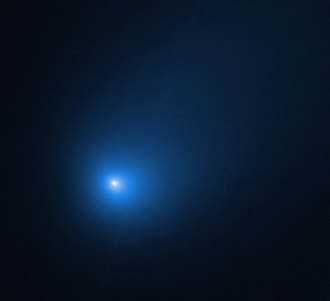
\includegraphics[width=0.95\textwidth]{static/borisov/hubble.jpg}
\caption[Borisov as seen by the NASA/ESA Hubble Space Telescope]{
Borisov as seen by the NASA/ESA Hubble Space Telescope. This image was
released on December 12, 2019, when the interloper was close to the Sun.
  }
  \label{fig:borisov_orbit}
\end{figure}







%
%...
%
%
%\subsection{Other candidates}
%
%...
